\documentclass[12pt,a4paper]{article}

\usepackage[in, plain]{fullpage}
\usepackage{array}
%\usepackage{../../../pas-math}
%\usepackage{../../../moncours}


%\usepackage{pas-cours}
%-------------------------------------------------------------------------------
%          -Packages nécessaires pour écrire en Français et en UTF8-
%-------------------------------------------------------------------------------
\usepackage[utf8]{inputenc}
\usepackage[frenchb]{babel}
\usepackage[T1]{fontenc}
\usepackage{lmodern}
\usepackage{textcomp}



%-------------------------------------------------------------------------------

%-------------------------------------------------------------------------------
%                          -Outils de mise en forme-
%-------------------------------------------------------------------------------
\usepackage{hyperref}
\hypersetup{pdfstartview=XYZ}
%\usepackage{enumerate}
\usepackage{graphicx}
\usepackage{multicol}
\usepackage{tabularx}
\usepackage{multirow}


\usepackage{anysize} %%pour pouvoir mettre les marges qu'on veut
%\marginsize{2.5cm}{2.5cm}{2.5cm}{2.5cm}

\usepackage{indentfirst} %%pour que les premier paragraphes soient aussi indentés
\usepackage{verbatim}
\usepackage{enumitem}
\usepackage[usenames,dvipsnames,svgnames,table]{xcolor}

\usepackage{variations}

%-------------------------------------------------------------------------------


%-------------------------------------------------------------------------------
%                  -Nécessaires pour écrire des mathématiques-
%-------------------------------------------------------------------------------
\usepackage{amsfonts}
\usepackage{amssymb}
\usepackage{amsmath}
\usepackage{amsthm}
\usepackage{tikz}
\usepackage{xlop}
%-------------------------------------------------------------------------------



%-------------------------------------------------------------------------------


%-------------------------------------------------------------------------------
%                    - Mise en forme avancée
%-------------------------------------------------------------------------------

\usepackage{ifthen}
\usepackage{ifmtarg}


\newcommand{\ifTrue}[2]{\ifthenelse{\equal{#1}{true}}{#2}{$\qquad \qquad$}}

%-------------------------------------------------------------------------------

%-------------------------------------------------------------------------------
%                     -Mise en forme d'exercices-
%-------------------------------------------------------------------------------
%\newtheoremstyle{exostyle}
%{\topsep}% espace avant
%{\topsep}% espace apres
%{}% Police utilisee par le style de thm
%{}% Indentation (vide = aucune, \parindent = indentation paragraphe)
%{\bfseries}% Police du titre de thm
%{.}% Signe de ponctuation apres le titre du thm
%{ }% Espace apres le titre du thm (\newline = linebreak)
%{\thmname{#1}\thmnumber{ #2}\thmnote{. \normalfont{\textit{#3}}}}% composants du titre du thm : \thmname = nom du thm, \thmnumber = numéro du thm, \thmnote = sous-titre du thm

%\theoremstyle{exostyle}
%\newtheorem{exercice}{Exercice}
%
%\newenvironment{questions}{
%\begin{enumerate}[\hspace{12pt}\bfseries\itshape a.]}{\end{enumerate}
%} %mettre un 1 à la place du a si on veut des numéros au lieu de lettres pour les questions 
%-------------------------------------------------------------------------------

%-------------------------------------------------------------------------------
%                    - Mise en forme de tableaux -
%-------------------------------------------------------------------------------

\renewcommand{\arraystretch}{1.7}

\setlength{\tabcolsep}{1.2cm}

%-------------------------------------------------------------------------------



%-------------------------------------------------------------------------------
%                    - Racourcis d'écriture -
%-------------------------------------------------------------------------------

% Angles orientés (couples de vecteurs)
\newcommand{\aopp}[2]{(\vec{#1}, \vec{#2})} %Les deuc vecteurs sont positifs
\newcommand{\aopn}[2]{(\vec{#1}, -\vec{#2})} %Le second vecteur est négatif
\newcommand{\aonp}[2]{(-\vec{#1}, \vec{#2})} %Le premier vecteur est négatif
\newcommand{\aonn}[2]{(-\vec{#1}, -\vec{#2})} %Les deux vecteurs sont négatifs

%Ensembles mathématiques
\newcommand{\naturels}{\mathbb{N}} %Nombres naturels
\newcommand{\relatifs}{\mathbb{Z}} %Nombres relatifs
\newcommand{\rationnels}{\mathbb{Q}} %Nombres rationnels
\newcommand{\reels}{\mathbb{R}} %Nombres réels
\newcommand{\complexes}{\mathbb{C}} %Nombres complexes


%Intégration des parenthèses aux cosinus
\newcommand{\cosP}[1]{\cos\left(#1\right)}
\newcommand{\sinP}[1]{\sin\left(#1\right)}


%Probas stats
\newcommand{\stat}{statistique}
\newcommand{\stats}{statistiques}
%-------------------------------------------------------------------------------

%-------------------------------------------------------------------------------
%                    - Mise en page -
%-------------------------------------------------------------------------------

\newcommand{\twoCol}[1]{\begin{multicols}{2}#1\end{multicols}}


\setenumerate[1]{font=\bfseries,label=\textit{\alph*})}
\setenumerate[2]{font=\bfseries,label=\arabic*)}


%-------------------------------------------------------------------------------
%                    - Elements cours -
%-------------------------------------------------------------------------------





%\makeatletter
%\renewcommand*{\@seccntformat}[1]{\csname the#1\endcsname\hspace{0.1cm}}
%\makeatother


%\author{Olivier FINOT}
\date{}
\title{Correction exercices démonstration}

%\graphicspath{./img/exos/}

%
%\rfoot{Page \thepage}

\graphicspath{{./img/exos/}}
\begin{document}
	
\maketitle

\vspace*{-3cm}
%
%\dominitoc
%
%\tableofcontents

%\chapter{Droites, segments et codage}
%\chap[num=2, color=red]{Droites, segments et codage}{Olivier FINOT, \today }

%\begin{myobj}
	\begin{itemize}
		
		\item Construire le symétrique d’un point ou d'une figure par rapport à une droite à la main où à l’aide d’un logiciel;
		\item Construire le symétrique d’un point ou d'une figure par rapport à un point, à la main où à l’aide d’un logiciel;
		\item Utiliser les propriétés de la symétrie axiale ou centrale;
		\item Identifier des symétries dans des figures.		
	\end{itemize}
\end{myobj}

\begin{mycomp}
	\begin{itemize}
		\item \kw{Chercher (Ch2)} :  s’engager    dans    une    démarche    scientifique, observer, questionner, manipuler, expérimenter (sur une feuille de papier, avec des objets, à l’aide de logiciels), émettre des hypothèses, chercher des exemples ou des contre-exemples, simplifier ou particulariser une situation, émettre une conjecture ;
		\item \kw{Raisonner (Ra3)} :  démontrer : utiliser un raisonnement logique et des règles établies (propriétés, théorèmes, formules) pour parvenir à une conclusion ;
		\item \kw{Communiquer (Co2)} :  expliquer à l’oral ou à l’écrit (sa démarche, son raisonnement, un calcul, un protocole   de   construction   géométrique, un algorithme), comprendre les explications d’un autre et argumenter dans l’échange ; 
		
	\end{itemize}
\end{mycomp}




\section*{Exercice 1}

\noindent \textbf{Je sais que} Benjamin a joué au football toute l'après-midi.\\
\textbf{Or} si je fais du sport alors je transpire.\\
\textbf{Donc} Benjamin transpire.\\

\noindent \textbf{Je sais que} Benjamin transpire.\\
\textbf{Or} si je sue alors je me lave.\\
\textbf{Donc} Benjamin va se laver.\\

\noindent \textbf{Je sais que} Benjamin va se laver.\\
\textbf{Or} si je me douche, alors je mets de l’eau partout dans la salle de bain.\\
\textbf{Donc} Benjamin va mettre de l'eau partout dans la salle de bain.\\

\noindent \textbf{Je sais que} Benjamin va mettre de l'eau partout dans la salle de bain.\\
\textbf{Or} si je mets de l’eau partout dans une pièce, alors maman me fait nettoyer les sols.\\
\textbf{Donc} Benjamin va nettoyer les sols de la salle de bain.\\

\section*{Exercice 2}

\noindent \textbf{Je sais que} La nuit est tombée.\\
\textbf{Or} S’il fait nuit, alors les chats sont gris.\\
\textbf{Donc} les chats sont gris.\\

\noindent \textbf{Je sais que} Carole chante très fort.\\
\textbf{Or} si je chante à tue-tête, alors mes voisins sont contents.\\
\textbf{Donc} Donc ses voisins sont contents.\\

\noindent \textbf{Je sais que} Les chats sont gris et les voisins de Carole sont contents.\\
\textbf{Or} si mes voisins sont heureux et que les chats sont gris, alors les poules chantent la Marseillaise.\\
\textbf{Donc} les poules chantent la Marseillaise.\\

\noindent \textbf{Je sais que} les poules chantent la Marseillaise.\\
\textbf{Or} si des poules chantent, alors elles ont les dents qui poussent.\\
\textbf{Donc} les poules auront des dents.\\

\begin{center}
	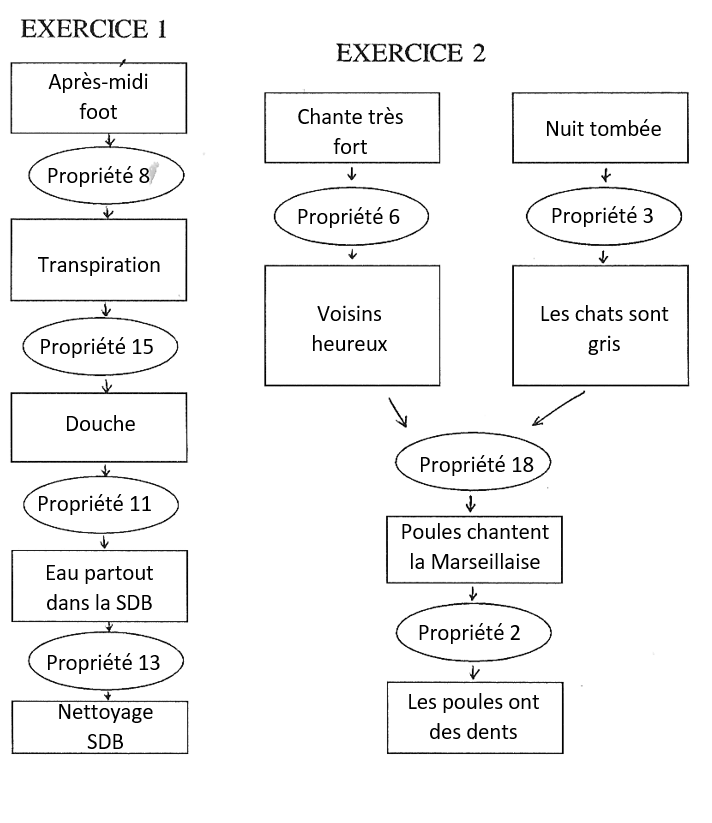
\includegraphics[scale=0.9]{demo_1-2}

\end{center}

\newpage

\section*{Exercice 3}

\noindent \textbf{Je sais que} Le Soleil brille.\\
\textbf{Or} s’il fait beau, alors je pars me promener.\\
\textbf{Donc} Léo va se promener.\\

\noindent \textbf{Je sais que} Léo va se promener.\\
\textbf{Or} si je sors de chez moi, alors je passe devant la boulangerie-pâtisserie à côté de chez moi.\\
\textbf{Donc} Léo va passer devant la boulangerie-pâtisserie.\\

\noindent \textbf{Je sais que} Léo a bien travaillé.\\
\textbf{Or} si je travaille bien, alors je reçois de l’argent de poche.\\
\textbf{Donc} Léo reçoit de l'argent de poche.\\

\noindent \textbf{Je sais que} Léo a de l'argent et qu'il passe devant la boulangerie-pâtisserie.\\
\textbf{Or} si j’ai de l’argent et que je passe devant une pâtisserie, alors je m’achète des petits gâteaux au chocolat.\\
\textbf{Donc} Léo va s'acheter des gâteaux.\\

\noindent \textbf{Je sais que} Léo va s'acheter des gâteaux.\\
\textbf{Or} si je mange des sucreries, alors j’ai des caries.\\
\textbf{Donc} Léo va avoir des caries.\\

\noindent \textbf{Je sais que} Léo va avoir des caries.\\
\textbf{Or} si j’ai des caries, alors je vais chez le dentiste.\\
\textbf{Donc} Léo aller chez le dentiste.\\

\begin{center}
	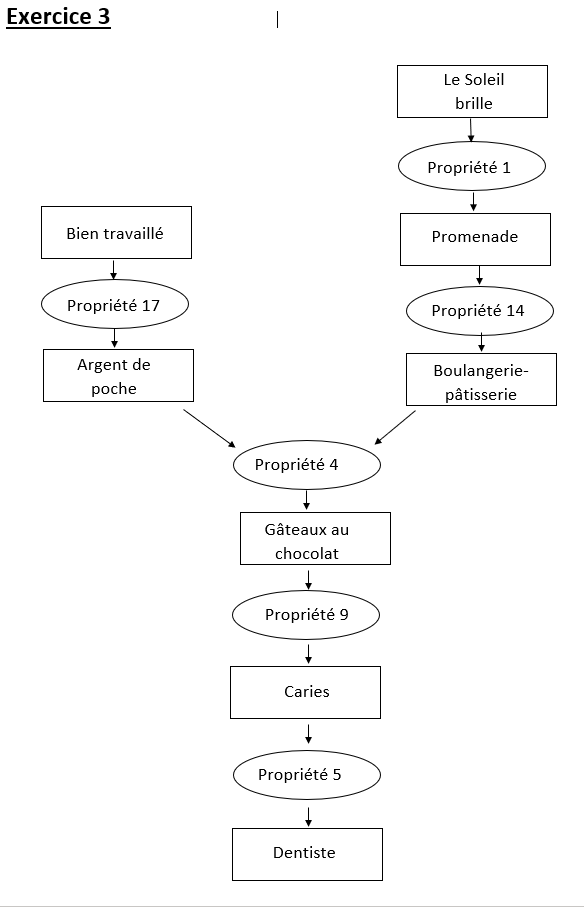
\includegraphics[scale=1]{demo_3}
	
\end{center}
\end{document}